%%
%%   This file is part of ICTP RegCM.
%%
%%   ICTP RegCM is free software: you can redistribute it and/or modify
%%   it under the terms of the GNU General Public License as published by
%%   the Free Software Foundation, either version 3 of the License, or
%%   (at your option) any later version.
%%
%%   ICTP RegCM is distributed in the hope that it will be useful,
%%   but WITHOUT ANY WARRANTY; without even the implied warranty of
%%   MERCHANTABILITY or FITNESS FOR A PARTICULAR PURPOSE.  See the
%%   GNU General Public License for more details.
%%
%%   You should have received a copy of the GNU General Public License
%%   along with ICTP RegCM.  If not, see <http://www.gnu.org/licenses/>.
%%

\newpage

\chapter{Model Equations}

The RegCM model solves a set of primitive dynamical equations describing
the atmospheric motion, with parametrizations for physical processes as per:

\begin{itemize}
  \item Radiation (Short Wave and Long Wave)
  \item Convection
  \item Turbolent Diffusion
  \item Moist (Clouds and Precipitation)
  \item Fluxes exchange with surface (Soil model and Ocean fluxes)
  \item Tracer transport and chemistry (Aerosols and full chemistry)
\end{itemize}

The dynamical equations are discretized using finite differences technique
on a three dimensional computation grid with fixed horizontal resolution
and terrain following vertical coordinate.

\section{Dynamics}
The model has three dynamical cores:

\begin{itemize}
\item Hydrostatic equation solver
\item Non-hydrostatic equation solver with pressure coordinate
\item Non-hydrostatic equation solver with height coordinate
\end{itemize}

The primitive equations for the three solvers are different and have different
prognostic variables used to identify the atmospheric state.

\subsection{Hydrostatic dynamical core}
The hydrostatic model dynamic equations and numerical discretization are
described by \cite{Grell_94}.

\subsubsection{Horizontal Momentum Equations}

\begin{gather}
\label{hydro_mom1}
  \frac{\partial{p^{\ast}u}}{\partial{t}} =
  -m^2 \left[ \frac{\partial{p^{\ast}uu/m}}{\partial{x}} + 
    \frac{\partial{p^{\ast}vu/m}}{\partial{y}} \right] -
    \frac{\partial{p^{\ast}u \dot{\sigma}}}{\partial{\sigma}}
      \\ \nonumber
      -mp^{\ast} \left[ \frac{\sigma}{\rho}
      \frac{\partial{p^{\ast}}}{\partial{x}} +
      \frac{\partial{\phi}}{\partial{x}} \right] +
  p^{\ast}fv + F_Hu + F_Vu \\
\label{hydro_mom2}
  \frac{\partial{p^{\ast}v}}{\partial{t}} = 
  -m^2 \left[ \frac{\partial{p^{\ast}uv/m}}{\partial{x}} +
    \frac{\partial{p^{\ast}vv/m}}{\partial{y}} \right] -
    \frac{\partial{p^{\ast}v\dot{\sigma}}}{\partial{\sigma}}
     \\ \nonumber
     -mp^{\ast} \left[ \frac{\sigma}{\rho}
         \frac{\partial{p^{\ast}}}{\partial{y}} +
      \frac{\partial{\phi}}{\partial{y}} \right]
  + p^{\ast}fu + F_Hv + F_Vv
\end{gather}

where $u$ and $v$ are the eastward and northward components of
velocity, $\phi$ is geopotential height, $f$ is the coriolis parameter,
$m$ is the map scale factor for the chosen projection, and $F_H$ and $F_V$
represent the effects of horizontal and vertical diffusion, and
$p^{\ast} = p_s-p_t$, i.e. the difference between surface and model top
pressure.  \\

In the equation \ref{hydro_mom1} - \ref{hydro_mom2}, $\dot{\sigma}$ is the total
derivative of the vertical coordinate $\sigma$ over time $t$:

\begin{equation}
\dot{\sigma} = {d\sigma \over dt}
\end{equation}

Moreover, given $T_v$ as the virtual temperature:

\begin{equation}
T_v = T \left( 1 + 0.608 Q_v \right)
\end{equation}

then

\begin{equation}
\frac{\sigma}{\rho} = \frac{RT_v}{(p^{\ast} + p_t/\sigma)}
\end{equation}

with $R$ the gas constant for dry air

\subsubsection{Continuity and Sigmadot $({\bf \dot{\sigma}})$ Equations}

The surface pressure is computed from the continuity equation:

\begin{eqnarray} \label{eq:continuity}
\frac{\partial{p^{\ast}}}{\partial{t}} = 
  -m^2 \left[ \frac{\partial{p^{\ast}u/m}}{\partial{x}} +
        \frac{\partial{p^{\ast}v/m}}{\partial{y}} \right] -
  \frac{\partial{p^{\ast}\dot{\sigma}}}{\partial{\sigma}}
\end{eqnarray}

The vertical integral of Equation~\ref{eq:continuity} is used to
compute the temporal variation of the surface pressure in the model,

\begin{eqnarray}
\label{intform}
  \frac{\partial{p^{\ast}}}{\partial{t}} = -m^2 \int_{0}^{1}
  {\left[ \frac{\partial{p^{\ast}u/m}}{\partial{x}} + 
    \frac{\partial{p^{\ast}v/m}}{\partial{y}} \right] d\sigma}
\end{eqnarray}

The surface pressure tendency from \ref{intform} is then used with the
the vertical integral of \ref{eq:continuity} to compute the vertical
velocity in sigma coordinates $(\dot{\sigma})$ at each
level in the model:

\begin{eqnarray}
  \dot{\sigma} = - \frac{1}{p^{\ast}} \int_{0}^{\sigma}{
    \left[ \frac{\partial{p^{\ast}}}{\partial{t}} +
    m^2 \left(\frac{\partial{p^{\ast}u/m}}{\partial{x}} +
                     \frac{\partial{p^{\ast}v/m}}{\partial{y}}
   \right) \right] d\sigma^\prime}
\end{eqnarray}

where $\sigma^\prime$ is a dummy variable of integration and
$\dot{\sigma}(\sigma=0)=0$, $\dot{\sigma}(\sigma=1)= 0$.

\subsubsection{Thermodynamic Equation and Equation for Omega ${\bf (\omega)}$}

The thermodynamic equation is

\begin{eqnarray}
\frac{\partial{p^{\ast}T}}{\partial{t}} = 
-m^2 \left[ \frac{\partial{p^{\ast}uT/m}}{\partial{x}} +
      \frac{\partial{p^{\ast}vT/m}}{\partial{y}} \right] -
      \frac{\partial{p^{\ast}T\dot{\sigma}}}{\partial{\sigma}} +
      \nonumber \\
  \frac{RT_v\omega}{c_{p}(\sigma + p_t/p_{\ast})} +
  \frac{p^{\ast}Q}{c_{p}} + F_HT + F_VT
\end{eqnarray}

where, given $c_{pd}$ the heat capacity of dry air and
$q_v$ the water vapor mixing ratio:

\begin{equation}
c_{p} = c_{pd} \left( 1 + 0.8q_v \right)
\end{equation}

$c_p$ is the specific heat for moist air at constant pressure, $Q$ is the
diabatic heating, $F_HT$ represents the effect of horizontal diffusion,
$F_VT$ represents the effect of vertical mixing and dry convective adjustment,
and $\omega$ is

\begin{equation}
  \omega = \frac{dp}{dt} = p^{\ast} \dot{\sigma} +
            \sigma \frac{dp^{\ast}}{dt}
\end{equation}

where:
  
\begin{eqnarray}
\frac{dp^{\ast}}{dt} =
   \frac{\partial{p^{\ast}}}{\partial{t}} + m
   \left[ u \frac{\partial{p^{\ast}}}{\partial{x}} +
          v \frac{\partial{p^{\ast}}}{\partial{y}} \right]
\end{eqnarray}

\subsubsection{Hydrostatic Equation}

The hydrostatic equation is used to compute the geopotential heights from
the virtual temperature $T_v$,

\begin{eqnarray}
\label{hydrostatic_equation}
\frac{\partial{\phi}}{\partial{\ln(\sigma + p_t / p^{\ast})}} =
-RT_v \left[ 1 + \frac{\sum{q_x}}{1 + q_v} \right]^{-1}
\end{eqnarray}

where $T_v = T(1 + 0.608q_v)$, $q_v$, is the water vapor mixing ratio, and
$q_x$ are the mixing ratios of all condensed water species.

\subsubsection{Split-explicit timestep for fast waves removal}

The vertical modes initialization is  described in \cite{Errico_88}.

The hydrostatic model equations above (\ref{hydro_mom1}-
\ref{hydrostatic_equation}) can be linearized about a state at rest,
with:

\begin{gather}
\label{reference_atm}
  \mean{u} = 0 \nonumber \\
  \mean{v} = 0 \nonumber \\
  T = \mean{T} \nonumber \\
  f_0 = \mean{f} \nonumber \\
  p^{\ast} = \mean{p}
\end{gather}

The linearized equations are:

\begin{gather}
  \label{linearized}
  \frac{\partial u}{\partial t} =
       f_0 v - \frac{\partial}{\partial x} (\phi^{\prime} +
       R\mean{T}\ln^{\prime}(\sigma p^{\ast} + p_t)) \\
  \frac{\partial v}{\partial t} =
       - f_0 u - \frac{\partial}{\partial y} (\phi^{\prime} +
       R\mean{T}\ln^{\prime}(\sigma p^{\ast} + p_t)) \\
  \frac{\partial T^\prime}{\partial t} =
     - \dot{\sigma} \frac{\partial \mean{T}}{\partial \sigma} +
     \frac{\kappa \mean{T}}{\sigma + \frac{p_t}{\mean{p}}}
     \frac{\omega}{\mean{p}} \\
  \label{2111a}
  \frac{\partial \ln\left(\frac{p^{\ast}}{\mean{p}}\right)}{\partial t} =
  -\int_0^1\left(\frac{\partial u}{\partial x} +
  \frac{\partial v}{\partial y} \right) d\sigma \\
  \label{2111b}
  \frac{\partial}{\partial t} \ln^{\prime}\left(\sigma p^{\ast} +
     p_t\right) = \frac{\sigma}{\sigma+\frac{p_t}{\mean{p}}}
        \frac{\partial}{\partial t}
        \ln\left(\frac{p^{\ast}}{\mean{p}}\right) \\
  \phi^{\prime} = \phi_S - R \int_0^1 T^{\prime}
    d \left[ \ln(\sigma \mean{p}+p_t)\right] -
    R \int_0^1 \mean{T} d \left[ \ln^{\prime}
    (\sigma p^{\ast}+p_t) \right] \\
  \dot{\sigma} = \sigma \int_0^1 \left(\frac{\partial u}{\partial x} +
  \frac{\partial v}{\partial y} \right) d\sigma -
  \int_0^{\sigma} \left(\frac{\partial u}{\partial x} +
  \frac{\partial v}{\partial y}\right) d\sigma^{\prime} \\
  \label{last_linearized}
  \frac{\omega}{\mean{p}} = \dot{\sigma} - \sigma
  \int_0^1 \left(\frac{\partial u}{\partial x} +
  \frac{\partial v}{\partial y}\right) d\sigma
\end{gather}

where

\begin{gather}
  T^{\prime}(x,y,t,\sigma) = T(x,y,t,\sigma) -
     \mean{T}(\sigma) \nonumber \\
  \ln^{\prime}(\sigma p^{\ast} + p_t) = \ln(\sigma p^{\ast} + p_t) -
    \ln(\sigma \mean{p} + p_t) \nonumber \\
  \kappa = \frac{R}{c_p} \nonumber
\end{gather}

Substituting now coordinates $u,v$ with horizontal vorticity $\zeta$ and
divergence $\delta$ defined as:

\begin{gather}
  \label{vorticity}
  \zeta = \frac{\partial v}{\partial x} -
          \frac{\partial u}{\partial y} \\
  \label{divergence}
        \delta = \frac{\partial u}{\partial x} +
                 \frac{\partial v}{\partial y}
\end{gather}

and defining the stream function $\psi$ and the velocity potential $\chi$
by:

\begin{gather}
  \left(\frac{\partial^2}{\partial x^2} +
        \frac{\partial^2}{\partial y^2}\right) \psi = 
        \nabla^2 \psi = \zeta \\
  \left(\frac{\partial^2}{\partial x^2} +
        \frac{\partial^2}{\partial y^2}\right) \chi = 
        \nabla ^2 \chi = \delta \\
  u = \frac{\partial \chi}{\partial x} -
      \frac{\partial \psi}{\partial y} \\
  v = \frac{\partial \chi}{\partial y} +
      \frac{\partial \psi}{\partial x}
\end{gather}

we obtain:

\begin{gather}
  \frac{\partial \zeta}{\partial t} = -f_0 \delta \\
  \frac{\partial \delta}{\partial t} = f_0 \zeta -
    \nabla^2\left[\phi^{\prime} + R \mean{T}
    \ln^{\prime}\left(\sigma p^{\ast} + p_t\right)\right] \\
  \label{2124}
  \frac{\partial T^{\prime}}{\partial t} = \bm{A} \delta \\
  \label{2125}
  \phi^{\prime} = \phi_S + R \bm{B} T^{\prime} +
      R \bm{C} \ln^{\prime} \left(\sigma p^{\ast} + p_t\right)
\end{gather}

where $\bm{A}, \bm{B}, \bm{C}$ are integral-differential operators in $\sigma$
function of $\mean{T}$ and $\frac{p_t}{\mean{p}}$.

Defining now the pseudo-geopotential $h$ as:

\begin{gather}
  \label{pseudogeop}
  h = \phi^{\prime} + R \mean{T} \ln^{\prime}
      \left(\sigma p^{\ast} + p_t\right)
\end{gather}

combining \ref{2125}, \ref{2124} and \ref{2111a}, we can derive time tendency
of this pseudo-geopotential $h$ as:

\begin{gather}
  \frac{\partial h}{\partial t} = - \tau(\delta)
\end{gather}

with $\tau$ is the integral $\sigma$-coordinate operator:

\begin{gather}
  \tau( ) = -R \bm{B}\bm{A}( ) + R \left( \bm{C} + \mean{T} \right)
    \frac{\sigma}{\sigma + \frac{p_t}{\mean{p}}}
    \int_0^1 ( ) d\sigma
\end{gather}

The complete nonlinear equations may be written as:

\begin{gather}
  \label{cmplnonlin1}
  \frac{\partial \zeta}{\partial t} = -f_0 \delta + N_{\zeta} \\
  \label{cmplnonlin2}
  \frac{\partial \delta}{\partial t} = f_0 \zeta -
     \nabla^2 h + N_{\delta} \\
  \label{cmplnonlin3}
  \frac{\partial h}{\partial t} = - \tau(\delta) + N_{h} \\
  \frac{\partial p^{\ast}}{\partial t} = -
     \int_0^1 \left(\frac{\partial p^{\ast}u}{\partial x} +
     \frac{\partial p^{\ast} v}{\partial y} \right) d\sigma
\end{gather}

where the non linear terms contains also horizontal variations of $f$.

If we now impose the conditions:

\begin{itemize}
  \item the primitive equations have slow behavior
  \item the time tendencies of the amplitudes of gravitational waves are
    negligible compared with other terms in the prognostic equations
  \item the linearized potential vorticity
    $\eta = \zeta - f_0 \tau^{-1}(h)$ is unchanged
\end{itemize}

we have:

\begin{gather}
  f_0 \zeta - \nabla^2 h = -N_{\delta} \\
  \frac{\partial}{\partial t}\left( f_0 \zeta - \nabla^2 h\right) = 0 \\
  \frac{\partial \eta}{\partial t} = 
   \frac{\partial \left(\zeta - f_0 \tau^{-1}(h)\right)}{\partial t} = 0
\end{gather}

The complete set of equations for the balance condition is:

\begin{gather}
  \label{balance_condition_1}
  \left(f_0^2 \tau^{-1} - \nabla^2\right) \zeta =
      -f_0\tau^{-1} N_{\delta} - \nabla^2 \eta \\
  \label{balance_condition_2}
  \left(f_0^2 \tau^{-1} - \nabla^2\right) \delta =
      \tau^{-1}\left(f_0 N_{\zeta} - \nabla^2 N_h \right) \\
  \label{balance_condition_3}
  h = \tau f_0^{-1}\left(\zeta - \eta\right)
\end{gather}

The equations \ref{balance_condition_1}, \ref{balance_condition_2} and
\ref{balance_condition_3} are solved iteratively, assuming a first guess if
the three fields, computing the $N_{(\zeta,\delta,h)}$ and then solving
them with those values. The process is repeated until convergence (smaller
time step).

Assuming:

\begin{gather}
  \zeta^N = \zeta^0 + \Delta \zeta \\
  \delta^N = \delta^0 + \Delta \delta \\
  h^N = h^0 + \Delta h
\end{gather}

the tendencies are:

\begin{gather}
  \frac{\partial \zeta}{\partial t} = -f_0 \delta^0 + N_{\zeta^0} \\
  \frac{\partial \delta}{\partial t} = f_0 \zeta^0 -
     \nabla^2 h^0 + N_{\delta^0} \\
  \frac{\partial h}{\partial t} = -\tau(\delta^0) + N_{h^0}
\end{gather}

then the changes to compute next timelevel are:

\begin{gather}
  \label{nextlev1}
  \left(f_0^2\tau^{-1}-\nabla^2\right) \Delta\zeta =
  -f_0 \tau^{-1} \left(f_0 \zeta^0-\nabla^2 h^0 + N_{\delta^0} \right) \\
  \label{nextlev2}
  \left(f_0^2\tau^{-1}-\nabla^2\right) \Delta\delta =
  \tau^{-1} \left(f_0 (-f_0 \delta^0 + N_{\zeta^0}) -
  \nabla^2(-\tau(\delta^0) + N_{h^0})\right) \\
  \label{nextlev3}
  \Delta h = \tau f_0^{-1} \Delta \zeta
\end{gather}

To solve the equations \ref{nextlev1}, \ref{nextlev2}, \ref{nextlev3} we need
to invert the three dimensional differential operator $f_0^2\tau^{-1}-\nabla^2$,
but being $\tau$ function only of $\sigma$ and $\nabla^2$ only of $x,y$, we can
separate horizontal and vertical coordinates.
In particular, we can use a transformation in terms of the eigenvectors of
$\tau$, which are called the vertical structure functions or vertical modes
of the linearized primitive equations \ref{linearized} - \ref{last_linearized}.
For the finite number of discrete $kz$ $\sigma$ levels, the operator $\tau^{-1}$
is defined as a $kz\times kz$ matrix withe the normal modes $\bm{z_i}$ as the
$kz$-dimensional vectors satisfying the equation:

\begin{gather}
  \left( g H_i - \tau \right) \bm{z_i} = 0
\end{gather}

where $H_i$ are the corresponding eigenvalues, called the equivalent depths,
because when the vertical profile $\mean{T}(\sigma)$ is statically stable the
values of $H_i$ are positive valued and bounded.

The problem has $kz$ independent solutions, and given as $\bm{Z}$ the
$kx\times kz$ matrix whose columns are the eigenvectors $\bm{z_i}$ and
$\bm{H}$ the diagonal matrix of correspondingly ordered $H_i$, it can
be rewritten as:

\begin{gather}
  g\bm{H}\bm{Z} = \tau \bm{Z}
\end{gather}

If we represent the three dimensional field $\zeta$, $\delta$ and $h$ as one
dimensional vectors of two dimensional fields:

\begin{gather}
  \bm{\zeta}(x,y,t) = (\zeta(x,y,\sigma_1,t),\zeta(x,y,\sigma_2,t),
         \dots,\zeta(x,y,\sigma_{kz},t))^\top \\
  \bm{\delta}(x,y,t) = (\delta(x,y,\sigma_1,t),\delta(x,y,\sigma_2,t),
         \dots,\delta(x,y,\sigma_{kz},t))^\top \\
  \bm{h}(x,y,t) = (h(x,y,\sigma_1,t),h(x,y,\sigma_2,t),
         \dots,h(x,y,\sigma_{kz},t))^\top
\end{gather}

having computed the $\bm{Z}$ matrix, we can transform from the $\sigma$
coordinates to the vertical-model amplitudes with:

\begin{gather}
  \label{hatz1}
  \hat{\bm{\zeta}} = \bm{Z^{-1}} \bm{\zeta} \\
  \label{hatz2}
  \hat{\bm{\delta}} = \bm{Z^{-1}} \bm{\delta} \\
  \label{hatz3}
  \hat{\bm{h}} = \bm{Z^{-1}} \bm{h} \\
  \nonumber \\
  \bm{\zeta} = \bm{Z} \hat{\bm{\zeta}} \\
  \bm{\delta} = \bm{Z} \hat{\bm{\delta}} \\
  \bm{h} = \bm{Z} \hat{\bm{h}}
\end{gather}

with the $\bm{I}$ identity matrix $kz\times kz$ as:

\begin{gather}
  \bm{I} = \bm{Z}\bm{Z^{-1}}
\end{gather}

In terms of the above defined vertical mode amplitudes, the complete
non-linear equations in \ref{cmplnonlin1} - \ref{cmplnonlin3} can be
rewritten as:

\begin{gather}
  \frac{\partial \hat{\zeta}_i}{\partial t} = - f_0 \hat{\delta}_i +
     \hat{N}_{\zeta_i} \\
  \frac{\partial \hat{\delta}_i}{\partial t} = f_0 \hat{\zeta}_i -
     \nabla^2 \hat{h}_i + \hat{N}_{\delta_i} \\
  \frac{\partial \hat{h}_i}{\partial t} = -g H_i \hat{\delta}_i +
     \hat{N}_{h_i}
\end{gather}

Ignoring the non-linear terms $N$, we can thus, for discrete $\sigma_i$,
replace the three dimensional operator $(f_0^2\tau^{-1} - \nabla^2)$ with
a set of two-dimensional operators $(\lambda_i - \nabla^2)$ where

\begin{gather}
  \lambda_i = \frac{f_0^2}{gH_i}
\end{gather}

which are the squared inverse of the Rossby radius of deformation
corresponding to the $H_i$ dephts.
The balanced fields are thus obtained by iterating:

\begin{gather}
  \label{to_be_iterated1}
  \left( \lambda_i - \nabla^2 \right) \Delta \hat{\zeta}_i =
     \frac{\lambda}{f_0} \frac{\partial \hat{\delta}}{\partial t} \\
  \label{to_be_iterated2}
  \left( \lambda_i - \nabla^2 \right) \Delta \hat{\delta}_i =
     \frac{\lambda}{f_0^2} \left( f_0 
     \frac{\partial \hat{\zeta}}{\partial t} -
     \nabla^2 \frac{\partial \hat{h}}{\partial t} \right) \\
  \label{to_be_iterated3}
  \Delta \hat{h}_i = f_0 \lambda^{-1} \Delta \hat{\zeta}_i
\end{gather}

Using the relations:

\begin{gather}
  \Delta \left( \ln p\right) = \int_0^1 \tau^{-1} \Delta h d\sigma \\
  p^N = p^0 \exp^{\left( \Delta \ln p \right)}
\end{gather}

the temperature changes can be computed as:

\begin{gather}
  \label{tchange}
  \Delta T = \frac{1}{R} \bm{B}^{-1} \left[ \Delta h - R
  \left( \bm{C} + \mean{T}\right) \ln \left(
  \frac{\sigma p^N + p_t}{\sigma p^0 + p_t}\right) \right]
\end{gather}

Defining now a shorter timestep $\hat{\Delta} t$, the sequence
to balance the dynamic fields and thus remove the fast wave components,
known the matrix $\bm{Z}$, are thus:

\begin{enumerate}
  \item \label{step1} Compute $\zeta$, $\delta$ and $h$ from the model
    variables $u$, $v$, $T$, $p^{\ast}$ at time $t$ using
    equation \ref{vorticity}, \ref{divergence} and
    \ref{pseudogeop}
  \item \label{step2} Compute $\hat{\zeta}$, $\hat{\delta}$, $\hat{h}$
    from $\zeta$, $\delta$ and $h$ using \ref{hatz1}, \ref{hatz2}
    and \ref{hatz3}
  \item Compute the new values of the prognostic variables
    $u$, $v$, $T$, $p^{\ast}$ at $t = t + \Delta t$ using
    model dynamic and physic
  \item Repeat the steps \ref{step1}, \ref{step2} for the new timestep
  \item Compute the tendencies of $\hat{\zeta}$, $\hat{\delta}$, $\hat{h}$
    using the two discrete timesteps and short timestep
    $\hat{\Delta} t$ as in:
    \begin{gather}
      \frac{\partial \hat{\zeta}}{\partial t} = 
      \left[ \frac{\left( \hat{\zeta}_{t+\hat{\Delta} t} -
           \hat{\zeta}_t \right)}{\hat{\Delta} t} \right] \\
      \frac{\partial \hat{\delta}}{\partial t} = 
      \left[ \frac{\left( \hat{\delta}_{t+\hat{\Delta} t} -
           \hat{\delta}_t \right)}{\hat{\Delta} t} \right] \\
      \frac{\partial \hat{h}}{\partial t} = 
      \left[ \frac{\left( \hat{h}_{t+\Delta t} -
           \hat{h}_t \right)}{\hat{\Delta} t} \right]
    \end{gather}
  \item Compute the right hand side of \ref{to_be_iterated1},
    \ref{to_be_iterated2}, \ref{to_be_iterated3}
  \item Solve the equations \ref{to_be_iterated1}, \ref{to_be_iterated2}
    for $\Delta \hat{\zeta}_i$ and $\Delta \hat{\delta}_i$
  \item Compute $\Delta \hat{h}_i$ using \ref{to_be_iterated3}
  \item Compute velocity modifications in terms of $\Delta \hat{\psi}$
    and $\Delta \hat{\chi}$ corresponding to the computed
    $\Delta \hat{\zeta}_i$ and $\Delta \hat{\delta}_i$ using the
    definitions of stream function and velocity potential
  \item Transform those to modifications in $\Delta u$ and $\Delta v$
    and $\Delta h$
  \item Compute $\Delta p$ using \ref{2111a} and \ref{2111b} or
    \cite{Daley} variational analysis
  \item Compute changes to $T$ using \ref{tchange}
  \item Compute updated fields and iterate
\end{enumerate}

\newpage

\subsection{Non-hydrostatic dynamical core with pressure vertical coordinate}
The non-hydrostatic model dynamic equations and numerical discretization are
described by \cite{Grell_94}.

\subsubsection{Model Equations}

Being $p^{\ast}$ constant in time, in the non-hydrostatic the continuity
equation no longer applies, thus the $DIV$ term appear in the equations
\ref{non-hydro-eq-first}-\ref{non-hydro-eq-last}:

\begin{gather}
\label{non-hydro-eq-first}
\frac{\partial{p^{\ast} u}}{\partial{t}} = -m^2 \left[ 
  \frac{\partial{p^{\ast} uu/m}}{\partial{x}} + 
\frac{\partial{p^{\ast} vu/m}}{\partial{y}}\right] -
  \frac{\partial{p^{\ast} u \dot{\sigma}}}{\partial{\sigma}} + 
  uDIV \\ \nonumber
  -\frac{mp^{\ast}}{\rho} \left[
    \frac{\partial{p^\prime}}{\partial{x}} -
    \frac{\sigma}{p^{\ast}}
    \frac{\partial{p^{\ast}}}{\partial{x}}
          \frac{\partial{p^\prime}}{\partial{\sigma}}\right] +
  p^{\ast}fv - p^{\ast} ew \cos\theta + D_u  \\
\frac{\partial{p^{\ast} v}}{\partial{t}}= -m^2 \left[ 
  \frac{\partial{p^{\ast} uv/m}}{\partial{x}} + 
  \frac{\partial{p^{\ast} vv/m}}{\partial{y}}\right] -
  \frac{\partial{p^{\ast} v \dot{\sigma}}}{\partial{\sigma}}+ 
  vDIV \\ \nonumber
  -\frac{mp^{\ast}}{\rho} \left[
    \frac{\partial{p^\prime}}{\partial{y}} -
    \frac{\sigma}{p^{\ast}}
    \frac{\partial{p^{\ast}}}{\partial{y}}
    \frac{\partial{p^\prime}}{\partial{\sigma}} \right] -
  p^{\ast}fu + p^{\ast} ew \sin\theta + D_v \\
\frac{\partial{p^{\ast} w}}{\partial{t}} = -m^2 \left[ 
  \frac{\partial{p^{\ast} uw/m}}{\partial{x}} + 
  \frac{\partial{p^{\ast} vw/m}}{\partial{y}}\right] -
  \frac{\partial{p^{\ast} w \dot{\sigma}}}{\partial{\sigma}} + 
  wDIV \\ \nonumber
  + p^{\ast}g\frac{\rho_0}\rho{}\left[
    \frac{1}{p^{\ast}}
    \frac{\partial{p^\prime}}{\partial{\sigma}} +
    \frac{T^{\prime}_{v}}{T} -
    \frac{T_0 p^\prime}{Tp_0} \right]
  -p^{\ast} g \left[\left(q_c+q_r\right)\right] \\ \nonumber
  + p^{\ast} e \left( u\cos\theta - v\sin\theta \right) + D_w \\
\frac{\partial{p^{\ast} p^\prime}}{\partial{t}} = -m^2 \left[ 
  \frac{\partial{p^{\ast} up^\prime/m}}{\partial{x}} + 
  \frac{\partial{p^{\ast} vp^\prime/m}}{\partial{y}}\right] -
  \frac{\partial{p^{\ast} p^\prime \dot{\sigma}}}{\partial{\sigma}} + 
  p^{\prime}DIV \\ \nonumber
  - m^2 p^{\ast} \gamma p \left[
    \frac{\partial{u/m}}{\partial{x}} -
    \frac{\sigma}{mp^{\ast}}
    \frac{\partial{p^{\ast}}}{\partial{x}}
    \frac{\partial{u}}{\partial{\sigma}} + 
    \frac{\partial{v/m}}{\partial{y}} -
    \frac{\sigma}{mp^{\ast}}
    \frac{\partial{p^{\ast}}}{\partial{y}}
    \frac{\partial{v}}{\partial{\sigma}} \right] \\ \nonumber
  + \rho_0 g \gamma p \frac{\partial{w}}{\partial{\sigma}} +
  p^{\ast} \rho_0 gw \\
\label{non-hydro-eq-last}
\frac{\partial{p^{\ast} T}}{\partial{t}} = -m^2 \left[
  \frac{\partial{p^{\ast} uT/m}}{\partial{x}} +
  \frac{\partial{p^{\ast} vT/m}}{\partial{y}} \right] -
  \frac{\partial{p^{\ast} T \dot{\sigma}}}{\partial{\sigma}} +
  TDIV \\ \nonumber
  +\frac{1}{\rho c_p}\left[p^{\ast}\frac{Dp^{\prime}}{Dt} -
  \rho_0gp^{\ast}w -D_{p^\prime}\right] +
  p^{\ast}\frac{\dot{Q}}{c_p} +D_T
\end{gather}

where:

\begin{eqnarray}
  DIV = m^2 \left[ \frac{\partial{p^{\ast}u/m}}{\partial{x}} +
    \frac{\partial{p^{\ast} v/m}}{\partial{y}} \right] +
    \frac{\partial{p^{\ast} \dot{\sigma}}}{\partial{\sigma}} \\
  \dot{\sigma} = - \frac{\rho_0g}{p^{\ast}}w -
                   \frac{m\sigma}{p^{\ast}}
       \frac{\partial{p^{\ast}}}{\partial{x}}u -
       \frac{m\sigma}{p^{\ast}}
       \frac{\partial{p^{\ast}}}{\partial{y}} v \\
   \tan \theta = - \cos \phi \frac{\partial{\lambda}/ \partial{y}}
          {\partial{\phi}/ \partial{x}} \\ \nonumber
         \phi = latitude \\ \nonumber
         \lambda = longitude \\
   \gamma = c_p / c_v
\end{eqnarray}

\subsubsection{Sound Waves}

For the non-hydrostatic equations, the acoustic wave terms are separated
from the slow varying terms and handled with a shorter time steps. The reduced
equations contain only interactions between momentum and pressure:

\begin{gather}
\frac{\partial{u}}{\partial{t}} + \frac{m}{\rho} \left[
    \frac{\partial{p^\prime}}{\partial{x}} -
    \frac{\sigma}{p^{\ast}}
    \frac{\partial{p^\ast}}{\partial{x}}
    \frac{\partial{p^\prime}}{\partial{\sigma}} \right] = S_u \\
\frac{\partial{v}}{\partial{t}} + \frac{m}{\rho} \left[
    \frac{\partial{p^\prime}}{\partial{y}} -
    \frac{\sigma}{p^{\ast}}
    \frac{\partial{p^\ast}}{\partial{y}}
    \frac{\partial{p^\prime}}{\partial{\sigma}} \right] = S_v \\
\frac{\partial{w}}{\partial{t}} - \frac{\rho_0}{\rho} 
  \frac{g}{p^\ast}\frac{\partial{p^\prime}}{\partial{\sigma}} +
  \frac{g}{\gamma} \frac{p^\prime}{p} = S_w \\
\frac{\partial{p^\prime}}{\partial{t}} + m^2 \gamma p \left[
    \frac{\partial{u/m}}{\partial{x}} -
    \frac{\sigma}{mp^\ast}
    \frac{\partial{p^\ast}}{\partial{x}}
    \frac{\partial{u}}{\partial{\sigma}} +
    \frac{\partial{v/m}}{\partial{y}} -
    \frac{\sigma}{mp^\ast}
    \frac{\partial{p^\ast}}{\partial{y}}
    \frac{\partial{v}}{\partial{\sigma}} \right] -
    \frac{\rho_0 g \gamma p}{p^\ast}
    \frac{\partial{w}}{\partial{\sigma}} - \rho_0 gw = S_{p^\prime}
\end{gather}

with $\gamma$ the ratio of the specific heats at constant pressure and volume.
During the small time-steps, the $S_x$ terms are kept constant (they contain
advection, diffusion, buoyancy and coriolis tendencies), and following the
semi-implicit scheme in \cite{Klemp_1978} we solve the above by recursion.
The step only depends on the horizontal grid size.

\subsection{Non-hydrostatic dynamical core with height vertical coordinate}

Given the definizion of the $\zeta$ vertical coordinate in \ref{h_coordinate},
the factor to transform the vertical derivatives in the new coordinate system
is thus:

\begin{eqnarray}
\sigma &=& 1 - \frac{\zeta}{H} \\
F_z &=& \frac{\partial \zeta}{\partial z} =
  \frac{\sigma}{B + h \frac{dG}{d\zeta}\sigma - H\sigma ln(\sigma)
  \frac{dB}{d\zeta}}
\end{eqnarray}

which allows for the generalized vertical velocity to be expressed as:

\begin{equation}
\dot{\zeta} = s = F_z \left[ w - 
              \left( u \frac{\partial h}{\partial x} +
                     v \frac{\partial h}{\partial y} \right) G \right]
\end{equation}

The model basic equation in 

\section{Physics parametrizations} \label{sec:physics}

\subsection{Radiation Scheme}

\noindent RegCM4 uses the radiation scheme of
the NCAR CCM3, which is described in \cite{Kiehl_96}.  Briefly, the solar
component, which accounts for the effect of ${\rm O_3}$, ${\rm H_2O}$, ${\rm
CO_2}$, and ${\rm O_2}$, follows the $\delta$-Eddington approximation of
\cite{Kiehl_96}.  It includes 18 spectral intervals from 0.2 to 5 $\mu {\rm m}$.
The cloud scattering and absorption parameterization follow that of
\cite{Slingo_89}, whereby the optical properties of the cloud droplets
(extinction optical depth, single scattering albedo, and asymmetry parameter)
are expressed in terms of the cloud liquid water content and an effective
droplet radius.  When cumulus clouds are formed, the gridpoint fractional cloud
cover is such that the total cover for the column extending from the
model-computed cloud-base level to the cloud-top level (calculated assuming
random overlap) is a function of horizontal gridpoint spacing.  The thickness of
the cloud layer is assumed to be equal to that of the model layer, and a
different cloud water content is specified for middle and low clouds.

\subsection{Land Surface Models}

\noindent {\bf BATS (default):} BATS is a surface package designed to describe
the role of vegetation and interactive soil moisture in modifying the
surface-atmosphere exchanges of momentum, energy, and water vapor (see
\cite{Dickinson_93} for details).  The model has a vegetation layer, a snow
layer, a surface soil layer, 10~cm thick, or root zone layer, 1-2~m thick, and a
third deep soil layer 3~m thick.  Prognostic equations are solved for the soil
layer temperatures using a generalization of the force-restore method of
\cite{Deardoff_78}.  The temperature of the canopy and canopy foilage is
calculated diagnostically via an energy balance formulation including sensible,
radiative, and latent heat fluxes.

The soil hydrology calculations include predictive equations for the water
content of the soil layers.  These equations account for precipitation,
snowmelt, canopy foiliage drip, evapotranspiration, surface runoff, infiltration
below the root zone, and diffusive exchange of water between soil layers.  The
soil water movement formulation is obtained from a fit to results from a
high-resolution soil model \cite{Dickinson_84} and the surface runoff rates are
expressed as functions of the precipitation rates and the degree of soil water
saturation.  Snow depth is prognostically calculated from snowfall, snowmelt,
and sublimation.  Precipitation is assumed to fall in the form of snow if the
temperature of the lowest model level is below 271~K.

Sensible heat, water vapor, and momentum fluxes at the surface are calculated
using a standard surface drag coefficient formulation based on surface-layer
similarity theory.  The drag coefficient depends on the surface roughness length
and on the atmospheric stability in the surface layer.  The surface
evapotranspiration rates depend on the availability of soil water.  \ac{BATS}
has 20 vegetation types (Table~\ref{landuse};  soil textures ranging from coarse
(sand), to intermediate (loam), to fine (clay);  and different soil colors
(light to dark) for the soil albedo calculations.  These are described in
\cite{Dickinson_86}. 

In the latest release version, additional modifications have been made to
\ac{BATS}in order to account for the subgrid variability of topography and
landcover using a mosaic-type approach \citep{Giorgi03b}.  Thismodification
adopts a regular fine-scale surface subgrid for eachcoarse model grid cell.
Meteorological variables are disaggregatedfrom the coarse grid to the fine
grid based on the elevationdifferences.  The \ac{BATS} calculations are then
performed separatelyfor each subgrid cell, and surface fluxes are reaggregated
onto thecoarse grid cell for input to the atmospheric model.
This parameterization showed a marked improvement in the representation ofthe
surface hydrological cycle in mountainous regions \citep{Giorgi03b}.
As a first augmentation, in \ac{RegCM4} two new land use types were added to
\ac{BATS} to represent urban and sub-urban environments. Urban development not
only modifies the surface albedo and alters the surface energy balance, but
also creates impervious surfaces with large effects on runoff and
evapotranspiration.
These effects can be described by modifying relevant properties of the land
surface types in the BATS package, such as maximum vegetation cover, roughness
length, albedo, and soil characteristics. For this purpose, we implemented the
parameters proposed in Table 1 of \cite{Kueppers_08}.

\noindent {\bf CLM (optional):} The Community Land Model (CLM; \cite{Oleson_08})
is the land surface model developed by the National Center of Atmospheric
Research (NCAR) as part of the Community Climate System Model (CCSM), described
in detail in \cite{Collins_06}.  CLM version 3.5 was coupled to RegCM for a more
detailed land surface description option.  CLM contains five possible snow
layers with an additional representation of trace snow and ten unevenly spaced
soil layers with explicit solutions of temperature, liquid water and ice water
in each layer.  To account for land surface complexity within a climate model
grid cell, CLM uses a tile or “mosaic” approach to capture surface
heterogeneity.  Each CLM gridcell contains up to four different land cover types
(glacier, wetland, lake, and vegetated), where the vegetated fraction can be
further divided into 17 different plant functional types.  Hydrological and
energy balance equations are solved for each land cover type and aggregated back
to the gridcell level.  A detailed discussion of CLM version 3 implemented in
RegCM3 and comparative analysis of land surface parameterization options is
presented in \cite{Steiner_09}.  Since CLM was developed for the global scale,
several input files and processes were modified to make it more appropriate for
regional simulations, including (1) the use of high resolution input data, (2)
soil moisture initialization, and (3) and an improved treatment of grid cells
along coastlines.  For the model input data, CLM requires several time-invariant
surface input parameters:  soil color, soil texture, percent cover of each land
surface type, leaf and stem area indices, maximum saturation fraction, and land
fraction \citep{Lawrence_07}.  Table~\ref{clm} shows the resolution for each
input parameter used at the regional scale in RegCM-CLM compared to resolutions
typically used for global simulations.  The resolution of surface input
parameters was increased for several parameters to capture surface heterogeneity
when interpolating to the regional climate grid.  Similar to \cite{Lawrence_07},
the number of soil colors was extended from 8 to 20 classes to resolve regional
variations.  The second modification was to update the soil moisture
initialization based on a climatological soil moisture average
\citep{Giorgi_89b} over the use of constant soil moisture content throughout the
grid generally used for global CLM.  By using a climatological average for soil
moisture, model spin-up time is reduced with regards to deeper soil layers.  The
third modification to the CLM is the inclusion of a mosaic approach for
gridcells that contain both land and ocean surface types.  With this approach, a
weighted average of necessary surface variables was calculated for land/ocean
gridcells using the land fraction input dataset.  This method provides a better
representation of coastlines using the high-resolution land fraction data
described in Table~\ref{clm}.  For a more detailed description of CLM physics
parameterizations see \cite{Oleson_04}.

\begin{table}
\centering
\caption{Land Cover/Vegetation classes}
\label{VegTypes}
\begin{tabular}{rl}
\hline
\hline
1.&Crop/mixed farming\\
2.&Short grass\\
3.&Evergreen needleleaf tree\\
4.&Deciduous needleleaf tree\\
5.&Deciduous broadleaf tree\\
6.&Evergreen broadleaf tree\\
7.&Tall grass\\
8.&Desert\\
9.&Tundra\\
10.&Irrigated Crop\\
11.&Semi-desert\\
12.&Ice cap/glacier\\
13.&Bog or marsh\\
14.&Inland water\\
15.&Ocean\\
16.&Evergreen shrub\\
17.&Deciduous shrub\\
18.&Mixed Woodland\\
19.&Forest/Field mosaic \\
20.&Water and Land mixture \\
\hline
\hline
\end{tabular}
\end{table}

\newpage

\begin{landscape}
\begin{table}
\centering
\caption{BATS vegetation/land-cover}
\label{landuse}
{\small
\begin{tabular}{lcccccccccccccccccccc}
\hline
\hline
\multicolumn{1}{c}{Parameter}&\multicolumn{20}{c}{Land Cover/Vegetation Type}\\
&1&2&3&4&5&6&7&8&9&10&11&12&13&14&15&16&17&18&19&20 \\ \hline Max fractional \\
vegetation
cover&0.85&0.80&0.80&0.80&0.80&0.90&0.80&0.00&0.60&0.80&0.35&0.00&0.80&0.00&0.00&0.80&0.80&0.80&0.80&0.80
\\ Difference between max\\ fractional vegetation \\ cover and cover at 269
K&0.6&0.1&0.1&0.3&0.5&0.3&0.0&0.2&0.6&0.1&0.0&0.4&0.0&0.0&0.2&0.3&0.2&0.4&0.4 \\
Roughness length (m)
&0.08&0.05&1.00&1.00&0.80&2.00&0.10&0.05&0.04&0.06&0.10&0.01&0.03&0.0004&0.0004&0.10&0.10&0.80&0.3&0.3
\\ Displacement height (m)
&0.0&0.0&9.0&9.0&0.0&18.0&0.0&0.0&0.0&0.0&0.0&0.0&0.0&0.0&0.0&0.0&0.0&0.0&0.0&0.0
\\ Min stomatal \\ resistence (s/m)  &45 &60 &80 &80 &120 &60 &60 &200 &80 &45
&150 &200 &45 &200 &200 &80 &120 &100&120&120  \\ Max Leaf Area Index
&6   &2   &6   &6   &6   &6   &6   &0   &6   &6   &6   &0   &6   &0   &0   &6
&6   &6 &6 &6    \\ Min Leaf Area Index            &0.5 &0.5 &5   &1   &1   &5
&0.5 &0   &0.5 &0.5 &0.5 &0   &0.5 &0   &0   &5   &1   &3  &0.5 &0.5   \\ Stem
(dead matter \\ area
index)&0.5&4.0&2.0&2.0&2.0&2.0&2.0&0.5&0.5&2.0&2.0&2.0&2.0&2.0&2.0&2.0&2.0&2.0&2.0&2.0
\\ Inverse square root of \\ leaf dimension
(m$^{-1/2}$)&10&5&5&5&5&5&5&5&5&5&5&5&5&5&5&5&5&5&5&5\\ Light sensitivity \\
factor (m$^2$
W$^{-1}$)&0.02&0.02&0.06&0.06&0.06&0.06&0.02&0.02&0.02&0.02&0.02&0.02&0.02&0.02&0.02&0.02&0.02&0.06&0.02&0.02
\\ Upper soil layer \\ depth (mm)     &100 &100 &100 &100 &100 &100 &100 &100
&100 &100 &100 &100 &100 &100 &100 &100 &100 &100 &100 &100  \\ Root zone soil\\
layer depth (mm) &1000 &1000 &1500 &1500 &2000 &1500 &1000 &1000 &1000 &1000
&1000 &1000 &1000 &1000 &1000 &1000 &1000 &2000 &2000 &2000  \\ Depth of total\\
soil (mm) &3000 &3000 &3000 &3000 &3000 &3000 &3000 &3000 &3000 &3000 &3000
&3000 &3000 &3000 &3000 &3000 &3000 &3000 &3000 &3000  \\ Soil texture type
&6   &6   &6   &6   &7   &8   &6   &3   &6   &6   &5   &12   &6   &6   &6   &6
&5   &6 &6 &0    \\ Soil color type    &5   &3   &4   &4   &4   &4   &4   &1
&3   &3   &2   &1   &5   &5   &5   &4   &3   &4 &4 &0    \\ Vegetation albedo
for \\ wavelengths $<$ 0.7 $\mu$ m
&0.10&0.10&0.05&0.05&0.08&0.04&0.08&0.20&0.10&0.08&0.17&0.80&0.06&0.07&0.07&0.05&0.08&0.06
&0.06 &0.06 \\ Vegetation albedo for \\ wavelengths $>$ 0.7 $\mu$ m
&0.30&0.30&0.23&0.23&0.28&0.20&0.30&0.40&0.30&0.28&0.34&0.60&0.18&0.20&0.20&0.23&0.28&0.24&0.18&0.18 \\
\hline
\hline
\end{tabular}
}
\end{table}
\end{landscape}
\newpage

\begin{table}
\centering
\caption{Resolution for CLM input parameters}
\begin{tabular}{ l  c c c   }
\hline
\hline
Input data & Grid Spacing & Lon range & Lat range \\
\hline
Glacier      & $0.05^{\circ}$ x $0.05^{\circ}$ & $\pm 179.975$ & $\pm 89.975$ \\Lake         & $0.05^{\circ}$ x $0.05^{\circ}$ & $\pm 179.975$ & $\pm 89.975$ \\
Wetland      & $0.05^{\circ}$ x $0.05^{\circ}$ & $\pm 179.975$ & $\pm 89.975$ \\
Land fraction& $0.05^{\circ}$ x $0.05^{\circ}$ & $\pm 179.975$ & $\pm 89.975$ \\
LAI/SAI      & $0.5^{\circ}$ x $0.5^{\circ}$   & $\pm 179.75$  & $\pm 89.75$  \\
PFT          & $0.5^{\circ}$ x $0.5^{\circ}$   & $\pm 179.75$  & $\pm 89.75$  \\
Soil color   & $0.05^{\circ}$ x $0.05^{\circ}$ & $\pm 179.975$ & $\pm 89.975$ \\
Soil texture & $0.05^{\circ}$ x $0.05^{\circ}$ & $\pm 179.975$ & $\pm 89.975$ \\
Max. sat. area  & $0.5^{\circ}$ x $0.5^{\circ}$ & $\pm 179.75$ & $\pm 89.75$  \\
\hline
\hline
\label{clm}
\end{tabular}
\end{table}

\subsection{Planetary Boundary Layer Scheme}
\subsubsection{Holtslag PBL}

The Holtslag planetary boundary layer scheme, developed by \cite{Holtslag_90},
is based on a nonlocal diffusion concept that takes into account
countergradient fluxes resulting from large-scale eddies in an unstable,
well-mixed atmosphere.  The vertical eddy flux within the PBL is given by

\begin{eqnarray}
F_c = -K_c \left( {\partial{C} \over \partial{z}} - \gamma_c \right)
\end{eqnarray}

where $\gamma_c$ is a ``countergradient'' transport term describing
nonlocal transport due to dry deep convection.  The eddy diffusivity is given by
the nonlocal formulation

\begin{eqnarray}
K_c = kw_tz \left( 1- {z \over h} \right)^2
\end{eqnarray}

where $k$ is the von Karman constant; $w_t$ is a turbulent convective
velocity that depends on the friction velocity, height, and the Monin--Obhukov
length;  and $h$ is the PBL height.

The countergradient term for temperature and water vapor is given by

\begin{eqnarray}
\label{eq:countergradient}
\gamma_c = C { {\phi_c}^0 \over w_t h}
\end{eqnarray}

where C is a constant equal to 8.5, and ${\phi_c}^0$ is the surface
temperature or water vapor flux. Equation~\ref{eq:countergradient} is applied
between the top of the PBL and the top of the surface layer, which is assumed to
be equal to $0.1h$. Outside this region and for momentum, $\gamma_c$ is assumed
to be equal to 0.  

For the calculation of the eddy diffusivity and countergradient terms, the PBL
height is diagnostically computed from

\begin{eqnarray}
  h = { {\rm {R_i}_{cr}} [u(h)^2 + v(h)^2] \over (g/\theta_s)[\theta_v(h)-\theta_s] }
\end{eqnarray}

where $u(h)$, $v(h)$, and $\theta_v$ are the wind components and the
virtual potential temperature at the PBL height, $g$ is gravity, ${\rm {R_i}_{cr}}$
is the critical bulk Richardson number, and $\theta_s$ is an appropriate
temperature of are near the surface.  Refer to \cite{Holtslag_90} and
\cite{Holtslag_93} for a more detailed description.

Compared to other schemes this formulation tends to produce relatively strong,
and often excessive, turbulent vertical transfer.
For example, after extensive testing, we found excessive vertical transfer
of moisture in the model resulting in low moisture amounts near the surface
and excessive moisture near the PBL top.

Therefore in order to ameliorate this problem, the countergradient term for
water vapor was removed in \ac{RegCM4}. Another problem of the Holtslag scheme
(at least in our implementation) is an excessive vertical transport of heat,
moisture and momentum in very stable conditions, such as during the winter in
northern hemisphere high latitude regions. For example we found that in such
conditions the scheme fails to simulate near surface temperature inversions.

This in turn leads to large warm winter biases (even > 10 degrees) over regions
such as Northern Siberia and Northern Canada. As an ad-hoc fix to address this
problem, in \ac{RegCM4} we implemented the following modification to the scheme:

\begin{itemize}
\item We first define “very stable” conditions within the Holtslag
parameterization as conditions in which the ratio of the height from the
surface over the Monin-Obhukov length is lower than 0.1.
\item When such conditions are found, we set to 0 the eddy diffusivity
and counter-gradient terms for all variables.
\end{itemize}

Preliminary tests showed that this modification reduces the warm bias in high
latitude winter conditions and allows the model to better capture surface
inversions. These modifications have thus been incorporated as default in the
\ac{RegCM4} code.

\subsubsection{The UW Turbulence Closure Model}

As an alternative to the Holtslag PBL, the University of Washington turbulence
closure model \citep{Grenier_01,Bretherton_04} has been coupled to RegCM.  The
development of this coupling, and its validation for western North America, is
described by \cite{OBrien_12a}, and validation over Europe is described by
\cite{Guettler_13}.  This parameterization was originally implemented to allow
RegCM to simulate stratocumulus and coastal fog
\citep{OBrien_12a,OBrien_12b}.

The UW model is a 1.5-order, local, down-gradient diffusion parametrization.
It will be referred to as a PBL model, but it has capabilities that allow it to
calculate vertical fluxes out side of the PBL as well as within;
\cite{Bretherton_04} refers to it as a moist turbulence parametrization.  As
with other 1$^{st}$-order models, such as the Holtslag model, the UW model
parameterizes turbulent fluxes as the product of a diffusivity and a gradient.
In contrast to 1$^{st}$-order models, however, the model prognostically
determines the turbulent kinetic energy (TKE, also referred to as $e$), and it
uses TKE to define the diffusivites. 

As with the Holtslag mode, diffusivity is defined as the product of a length
scale and a velocity scale, though the velocity scale is defined as the square
root of local TKE rather than the convective velocity scale. The length scale
is the UW model's master length scale, either $l = \kappa z$ or $l = kz/(1 +
kz/\lambda)$ (this can be set in the RegCM configuration file), multiplied by a
correction factor that depends on local stability\footnote{The correction
  factors are called the stability functions $S_{h,m}$, which are defined in
\cite{Galperin_88}}, and the velocity scale is the square root of twice the
TKE.

The boundary layer height in the UW model is defined as the first level where
the expression $N(z)^2 l(z)^2$ (where $N$ is the Brunt-V\"{a}is\"{a}l\"{a}
frequency, $N^2 = \frac{g}{\theta_v}\frac{\partial \theta_v}{\partial z}$)
exceeds half of the negative of its layer-mean value.  Since the flux of
buoyancy, $b$, can be written as $\overline{w'b'} = -K_h \frac{\partial
b}{\partial z}$, and it can be shown that $N^2 = \frac{\partial b}{\partial
z}$, $N^2$ can be viewed as being proportional to the local buoyancy flux in
the UW model.  In this interpretation, this condition for PBL top (or the top
of any turbulent layer) can be approximately viewed as a ``condition that the
buoyancy flux anywhere in the interior of a convective layer not be more
negative than -0.5 of the layer-mean buoyancy flux" \citep{Bretherton_04}.  In
other words for an unstable PBL, the PBL ends approximately when the virtual
potential temperature profile becomes so stable that the buoyancy flux is
opposite to and half as strong as the mean buoyancy flux below.  This condition
for the height of the PBL can be encapsulated in the following implicit
equation, where the $z$ and $h$ values are restricted to lie on the model's
vertical grid:

\begin{equation}\label{uwheight}
N^2(h)l^2(h) = -\frac{1}{2}\frac{1}{h}\int_{0}^{h}N^2(z)l^2(z)\cdot dz 
\end{equation}

The diffusivity of scalar quantities and momentum at a given height, $z$, are
given as $K_{h,m}(z) = l(z) S_{h,m}(z) \sqrt{2 e}$.  The TKE budget equation is
solved at each time step according to equation~\ref{tkeeqn} (where the shear
frequency, $S_f = \sqrt{(\frac{\partial u }{\partial z})^2 + (\frac{\partial v
}{\partial z})^2}$), which is the balance of buoyancy ($B$), shear ($S$),
transport ($T$), and dissipation ($D$) terms.  Following \cite{Grenier_01},
the TKE diffusivity, $K_e$, is set as 5 times the eddy diffusivity, $K_m$.  The
RegCM dynamical core has been modified to account for horizontal transport
(i.e.~advection and diffusion) of TKE when the UW model is active.

\begin{subequations}\label{tkeeqn}
\begin{align}
\frac{\partial e}{\partial t}\Bigr\rvert_{BL}&= -K_h N^2 + K_m {S_f}^2 + \frac{\partial}{\partial z}[K_e \frac{\partial e}{\partial z}] - \frac{e^{\frac{3}{2}}}{l}\\
\frac{\partial e}{\partial t}\Bigr\rvert_{BL}&= B + S + T - D
\end{align}
\end{subequations}

The UW model treats TKE and diffusivity at the surface and the PBL top
specially.  At the surface, TKE is diagnosed as $e_0 = B u_{*}^2$, where $B$ is
a constant.  At the PBL top (the temperature inversion), diffusivity for all
quantities is set as $K_X = w_e \Delta_{inv}z$.  The entrainment flux, which
uses the Turner-Deardorff formulation, is set as $w_e = \frac{A U}{R_i}$, where
$A$ is the entrainment efficiency\footnote{The entrainment efficiency is
  partially determined by the mixture of clear and cloudy air that happens at
the inversion top: \cite{Grenier_01} takes special care to develop a
parametrization for A that includes `evaporative enhancement' effects for cases
when a cloudy-clear mixture of air is more dense than its surroundings.}, $U$
is a scale velocity, and $R_i$ is a bulk Richardson number.  The UW model
specifies the bulk Richardson number as $R_i = \frac{L \Delta b}{U^2}$, with $U
= \sqrt{e_{inv}}$, and $L = l$ as the master length scale.  It is assumed that
the PBL does not entrain or detrain TKE.

The UW model accounts for the production of turbulence by cloud-top radiative
cooling, which is a critical difference from the Holtslag PBL.  If a turbulent
layer (e.g.~the PBL) is cloud-topped, then a term is added to the TKE budget
equation: $\frac{\partial e}{\partial t}\Bigr\rvert_{RAD} = \frac{g \Delta
F_{lw}}{C_p\rho \Pi \theta_v}\rvert_{inv}$, where $\Delta F_{lw}$ is the jump
in long-wave flux at cloud-top.  This term is crucial for ensuring that
turbulence is produced in the otherwise-stable regions where stratocumulus
exist.

The UW model is written specifically to deal with moist thermodynamic processes
(i.e.~mixing between clear and cloudy air): its core prognostic equations are
written to predict liquid water potential temperature, $\theta_l$, total water
mixing ratio, $Q$, and momentum, $u_i$.  The use of these variables ensures
that enthalpy and water are explicitly conserved when mixing between clear and
cloudy parcels of air; care has to be taken otherwise (when using $\theta$ and
$q$) to ensure conservation in this situation.

At each model timestep, the UW model does the following: determines the
boundary layer height, $h$, calculates the surface TKE,predicts the change in
TKE due to PBL processes, determines the diffusivities at each height, and
predicts the change in each prognostic quantity due to vertical convergence of
turbulent fluxes.  The full set of equations that the UW PBL model solves at
each time step, including equations~\ref{uwheight} and \ref{tkeeqn}, follows:

\begin{subequations}\label{uwmodel}
\begin{align}
\frac{\partial u_i}{\partial t}\Bigr\rvert_{BL} &= \frac{\partial}{\partial z}[\kappa z S_m(z) \sqrt{2 e(z)} \frac{\partial u_i}{\partial z}]\label{uwmodela} \\
\frac{\partial \theta_l}{\partial t}\Bigr\rvert_{BL} &= \frac{\partial}{\partial z}[\kappa z S_h(z) \sqrt{2 e(z)} \frac{\partial \theta_l}{\partial z}]\label{uwmodelb} \\
\frac{\partial Q}{\partial t}\Bigr\rvert_{BL} &= \frac{\partial}{\partial z}[\kappa z S_h(z) \sqrt{2 e(z)} \frac{\partial Q}{\partial z}]\label{uwmodelc} \\
\frac{\partial \chi_j}{\partial t}\Bigr\rvert_{BL} &= \frac{\partial}{\partial z}[\kappa z S_h(z) \sqrt{2 e(z)} \frac{\partial \chi_j}{\partial z}]\label{uwmodeld} 
\end{align}
\end{subequations}

\subsection{Convective Precipitation Schemes}

Convective precipitation is computed using one of three schemes: (1)
Modified-Kuo scheme \cite{Anthes_77}; (2) Grell scheme \cite{Grell_93}; and (3)
MIT-Emanuel scheme \citep{Emanuel_91,Emanuel_99}. In addition, the Grell
parameterization is implemented using one of two closure assumptions: (1) the
Arakawa and Schubert closure \cite{Grell_94} and (2) the Fritsch and Chappell
closure \cite{Fritsch_80}, hereafter refered to as AS74 and FC80,
respectively.\\

\noindent{
\begin{enumerate}
\item {\bf Kuo Scheme:}  Convective activity in the Kuo scheme is
initiated when the moisture convergence $M$ in a column exceeds a given
threshold and the vertical sounding is convectively unstable. A fraction of the
moisture convergence $\beta$ moistens the column and the rest is converted into
rainfall $P^{CU}$ according to the following relation:

\begin{eqnarray}
P^{CU}&=&M(1-\beta).
\label{eqn_model:KUOppt}
\end{eqnarray}

$\beta$ is a function of the average relative humidity $\overline{RH}$ of the
sounding as follows:

\begin{eqnarray}
\beta&=&\left\{
  \begin{array}
  {r@{\quad\quad}l} 2(1-\overline{RH}) & \overline{RH}\ge 0.5 \\
  1.0 & \mbox{otherwise}
  \end{array} 
  \right\}
\label{eqn_model:Bfact}
\end{eqnarray}

Note that the moisture
convergence term includes only the advective tendencies for water vapor.
However, evapotranspiration from the previous time step is indirectly included
in $M$ since it tends to moisten the lower atmosphere. Hence, as the
evapotranspiration increases, more and more of it is converted into rainfall
assuming the column is unstable. The latent heating resulting from condensation
is distributed between the cloud top and bottom by a function that allocates the
maximum heating to the upper portion of the cloud layer. To eliminate numerical
point storms, a horizontal diffusion term and a time release constant are
included so that the redistributions of moisture and the latent heat release are
not performed instantaneously \citep{Giorgi_89b, Giorgi_91c}. \\

\item {\bf Grell Scheme:} The Grell scheme \cite{Grell_93}, similar
to the AS74 parameterization, considers clouds as two steady-state circulations:
an updraft and a downdraft. No direct mixing occurs between the cloudy air and
the environmental air except at the top and bottom of the circulations. The mass
flux is constant with height and no entrainment or detrainment occurs along the
cloud edges. The originating levels of the updraft and downdraft are given by
the levels of maximum and minimum moist static energy, respectively. The Grell
scheme is activated when a lifted parcel attains moist convection. Condensation
in the updraft is calculated by lifting a saturated parcel. The downdraft mass
flux ($m_0$) depends on the updraft mass flux ($m_b$) according to the following
relation:

\begin{eqnarray}
m_0=\frac{\beta I_1}{I_2}m_b
\end{eqnarray}

where
$I_1$ is the normalized updraft condensation, $I_2$ is the normalized downdraft
evaporation, and $\beta$ is the fraction of updraft condensation that
re-evaporates in the downdraft. $\beta$ depends on the wind shear and typically
varies between 0.3 and 0.5. Rainfall is given by

\begin{eqnarray}
P^{CU}&=&I_1m_b(1-\beta)
\label{eqn_model:GCCppt}
\end{eqnarray}

Heating and
moistening in the Grell scheme are determined both by the mass fluxes and the
detrainment at the cloud top and bottom. In addition, the cooling effect of
moist downdrafts is included.

Due to the simplistic nature of the Grell scheme, several closure assumptions
can be adopted. RegCM4's earlier version directly implements the
quasi-equilibrium assumption of AS74. It assumes that convective clouds
stabilize the environment as fast as non-convective processes destabilize it as
follows:

\begin{eqnarray}
m_b=\frac{ABE''-ABE}{NA\Delta t}
\label{eqn_model:closureAS}
\end{eqnarray}

where $ABE$ is the buoyant energy
available for convection, $ABE''$ is the amount of buoyant energy available for
convection in addition to the buoyant energy generated by some of the
non-convective processes during the time interval $\Delta t$, and $NA$ is the
rate of change of $ABE$ per unit $m_b$. The difference $ABE''-ABE$ can be
thought of as the rate of destabilization over time $\Delta t$. $ABE''$ is
computed from the current fields plus the future tendencies resulting from the
advection of heat and moisture and the dry adiabatic adjustment.

In the latest RegCM4 version, by default, we use a stability based closure
assumption, the FC80 type closure assumption, that is commonly implemented in
GCMs and RCMs. In this closure, it is assumed that convection removes the $ABE$
over a given time scale as follows:

\begin{eqnarray}
m_b=\frac{ABE}{NA \tau}
\label{eqn_model:closureFC}
\end{eqnarray}

where $\tau$ is the $ABE$ removal time scale.

The fundamental difference between the two assumptions is that the AS74 closure
assumption relates the convective fluxes and rainfall to the tendencies in the
state of the atmosphere, while the FC80 closure assumption relates the
convective fluxes to the degree of instability in the atmosphere. Both schemes
achieve a statistical equilibrium between convection and the large-scale
processes.

A number of parameters present in the scheme can be used to optimize its
performance, and \cite{Giorgi_93c} discusses a wide range of sensitivity
experiments. We found that the parameter to which the scheme is most sensitive
is by and large the fraction of precipitation evaporated in the downdraft
(Peff, with values from 0 to 1), which essentially measures the precipitation
efficiency. Larger values of Peff lead to reduced precipitation.

\item {\bf MIT-Emanuel scheme:} 
More detailed descriptions can be found
in \citet{Emanuel_91} and\citet{Emanuel_99}.  The scheme assumes that the
mixing in clouds ishighly episodic and inhomogeneous (as opposed to a
continuousentraining plume) and considers convective fluxes based on
anidealized model of sub-cloud-scale updrafts and downdrafts.Convection is
triggered when the level of neutral buoyancy is greaterthan the cloud base
level.  Between these two levels, air is liftedand a fraction of the condensed
moisture forms precipitation while theremaining fraction forms the cloud.  The
cloud is assumed to mix withthe air from the environment according to a
uniform spectrum ofmixtures that ascend or descend to their respective levels
of neutralbuoyancy.  The mixing entrainment and detrainment rates are
functionsof the vertical gradients of buoyancy in clouds.  The fraction of
thetotal cloud base mass flux that mixes with its environment at eachlevel
is proportional to the undiluted buoyancy rate of change withaltitude.  The
cloud base upward mass flux is relaxed towards thesub-cloud layer quasi
equilibrium.

In addition to a more physical representation of convection, the MIT-Emanuel
scheme offers several advantages compared to theother RegCM4 convection
options.  For instance, it includes aformulation of the auto-conversion of
cloud water into precipitationinside cumulus clouds, and ice processes are
accounted for by allowingthe auto-conversion threshold water content to be
temperaturedependent.  Additionally, the precipitation is added to a
single,hydrostatic, unsaturated downdraft that transports heat and
water. Lastly, the MIT-Emanuel scheme considers the transport of passive
tracers.

The MIT scheme is the most complex of the three and also includes a number of
parameters that can be used to optimize the model performance in different
climate regimes. Differently from the Grell scheme, however, test experiments
did not identify a single parameter to which the model is most sensitive.
\end{enumerate}


A major augmentation in \ac{RegCM4} compared to previous versions of the model
is the capability of running different convection schemes over land and ocean,
a configuration which we refer to as “mixed convection”. Extensive test
experiments showed that different schemes have different performance over
different regions, and in particular over land vs. ocean areas.

For example, the MIT scheme tends to produce excessive precipitation over land
areas, especially through the occurrence of very intense individual
precipitation events.

In other words, once the scheme is activated, it becomes difficult to
“decelerate”. Conversely, we found that the Grell scheme tends to produce
excessively weak precipitation over tropical oceans.

These preliminary tests suggested that a mixed convection approach by which,
for example, the MIT scheme is used over oceans and the Grell scheme over
land, might be the most suitable option to pursue, and therefore this option
was added to the model.

\subsection{Large-Scale Precipitation Scheme}

Subgrid Explicit Moisture
Scheme (SUBEX) is used to handle nonconvective clouds and precipitation resolved
by the model.  This is one of the new components of the model.  SUBEX accounts
for the subgrid variability in clouds by linking the average grid cell relative
humidity to the cloud fraction and cloud water following the work of
\cite{Sundqvist_89}.  

The fraction of the grid cell covered by clouds, $FC$, is determined by,

\begin{eqnarray}
FC = \sqrt{ { {RH - RH_{min}} \over {RH_{max} - RH_{min} }} }
\end{eqnarray}

where ${RH_{min}}$ is the relative humidity threshold at which clouds
begin to form, and ${RH_{max}}$ is the relative humidity where $FC$ reaches
unity.  $FC$ is assumed to be zero when RH is less than ${RH_{min}}$ and unity
when RH is greater than ${RH_{max}}$.  

Precipitation $P$ forms when the cloud water content exceeds the autoconversion
threshold ${Q^{th}}_c$ according to the following relation:

\begin{eqnarray}
P = C_{ppt}(Q_c/FC - {{Q_c}^{th}})FC
\end{eqnarray}

where $1/C_{ppt}$ can be considered the characteristic time for which
cloud droplets are converted to raindrops.  The threshold is obtained by scaling
the median cloud liquid water content equation according to the following:

\begin{eqnarray}
{Q^{th}}_c = C_{acs} 10^{-0.49 + 0.013T}
\end{eqnarray}

where $T$ is temperature in degrees Celsius, and $C_{acs}$ is the
autoconversion scale factor.  Precipitation is assumed to fall instantaneously.

SUBEX also includes simple formulations for raindrop accretion and evaporation.
The formulation for the accretion of cloud droplets by falling rain droplets is
based on the work of \cite{Beheng_94} and is as follows:

\begin{eqnarray}
P_{acc} = C_{acc} Q P_{sum}
\end{eqnarray}

where $P_{acc}$ is the amount of accreted cloud water, $C_{acc}$ is
the accretion rate coefficient, and $P_{sum}$ is the accumulated precipitation
from above falling through the cloud.  

Precipitation evaporation is based on the work of \cite{Sundqvist_89} and is as
follows

\begin{eqnarray}
P_{evap} = C_{evap} (1-RH) {P^{1/2}}_{sum}
\end{eqnarray}

where $P_{evap}$ is the amount of evaporated precipitation, and
$C_{evap}$ is the rate coefficient.  For a more detailed description of SUBEX
and a list of the parameter values refer to \cite{Pal_00}. 

Traditionally, \ac{RegCM3} has shown a tendency to produce excessive
precipitation, especially at high resolutions, and optimizations of 
the in-cloud liquid water threshold for the activation of the autoconversion
term $Qcth$ and the rate of sub-cloud evaporation $Cevap$ parameters have
proven effective in ameliorating this problem: greater values of $Qth$ and
$Cevap$ lead to decreased precipitation amounts.

\subsection{The new cloud microphysics scheme}

The new scheme is built upon the European Centre for Medium Weather Forecast's Integrated Forecast System (IFS) (\citet{tiedtke:93}, \citet{tompkins:07}),
\citet{gmd-9-2533-2016}. \\
In the new scheme some important achievement have been added:
\begin{itemize}
\item Liquid and ice water content are independent, allowing the existence of supercooled liquid water and mixed-phase cloud.
\item Rain and snow now precipitate with a fixed, finite, terminal fall speed and can be then advected by the three dimensional wind.
\item The new scheme solves implicitly 5 prognostic equations for water vapor, cloud liquid water, rain, ice and snow. It is also easily suitable for a larger number of variables. Water vapor $q_v$, cloud liquid water $q_l$, rain $q_r$, ice $q_i$ and snow $q_s$ are all expressed in terms of the grid-mean mixing ratio.
\item A check for the conservation of enthalpy and of total moisture is en- sured at the end of each timestep.
\end{itemize}
The governing equation for each variable is:
\begin{equation}
\frac{\partial q_x}{\partial t}= S_x +\frac{1}{\rho}\frac{\partial}{\partial z}(\rho V_x q_x)
\end{equation}
The local variation of the mixing ratio $q_x$ of the variable $x$ is given by the sum of $S_x$, that contains the net sources and sinks of $q_x$ through 
\begin{figure} [htpb!]% Inline image example
\begin{center}
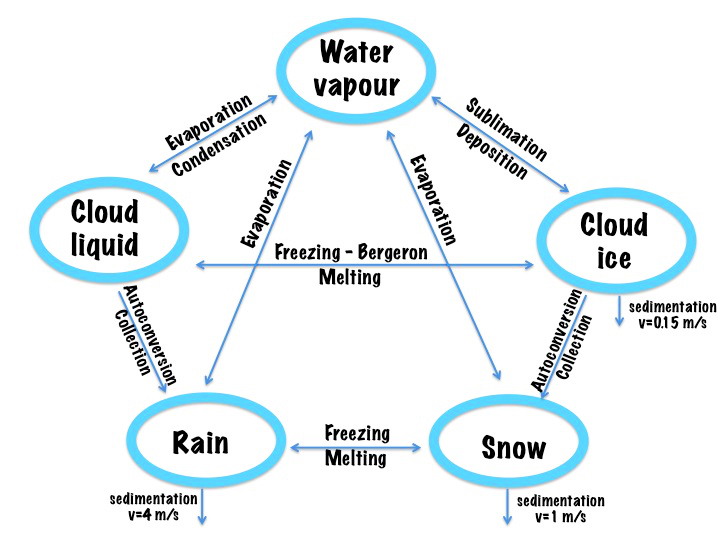
\includegraphics[width=0.6\textwidth]{scheme_var2.jpg}
\end{center}
\caption{\small Schematics of the new scheme, showing the 5 prognostic variables and  how they are related to each other through microphysical processes}
\label{fig:newscheme}
\end{figure}
\noindent microphysical properties (i.e. condensation, evaporation, auto-conversion, melting...), and the sedimentation term, that is a function of the fall speed $V_x$ that has a fixed value for each cloud variable. 
To solve the equations the upstream approach is used.  The sources and sinks contributors are divided in two groups according to the duration of the process they describe: processes that are considered to be fast relative to the timestep of the model are treated implicitly while slow processes are treated explicitly. The processes taken into account (shown in Fig.~\ref{fig:newscheme})) are the microphysical pathways between the 5 considered variables: condensation, autoconversion, evaporation, collection for the warm clouds, and autoconversion, freezing, melting, deposition, evaporation for the cold clouds.\\
For each microphysical pathway the change of phase is associated with a release or an absorption of latent heat, that has a significant impact on the temperature budget.
The impact is calculated using the conservation of liquid water temperature $T_L$ defined as:
\begin{equation}
T_L=T-\frac{L_v}{C_p}(q_l+q_r)-\frac{L_s}{C_p}(q_i+q_s).
\end{equation}
Being that $\frac{dT_L}{dt}=0$, the rate of change of the temperature is  given by the following equation:
\begin{equation}
\frac{\partial T}{\partial t}=\sum_{x=1}^m\frac{L(x)}{C_p}\Big(\frac{dq_x}{dt}-D_{q_x}-\frac{1}{\rho}\frac{\partial}{\partial z}(\rho V_x q_x)\Big)
\end{equation}
where $L(x)$ is the latent heat (of fusion or evaporation depending on the processes considered), $D_{q_x}$ is the convective detrainment and the third term in the brackets is the sedimentation term.\\
At the end of each timestep a routine checks the conservation of the total water and of the moist static energy $h=C_P T+gz+ Lq_x$.

\subsection{Ocean flux Parameterization}

\ac{BATS} uses standard Monin-Obukhov similarity relations to compute the
fluxes with no
special treatment of convective and very stable conditions.  In addition, the
roughness length is set to a constant, i.e. it is not a function of wind and
stability.  

The Zeng scheme describes all stability conditions and
includes a gustiness velocity to account for the additional flux induced by
boundary layer scale variability. Sensible heat (${\rm SH}$), latent heat (${\rm
LH}$), and momentum ($\tau$) fluxes between the sea surface and lower atmosphere
are calculated using the following bulk aerodynamic algorithms,
    
\begin{eqnarray}
\tau = \rho_a {u_{\ast}}^2 ({u_{x}}^2 + {u_{y}}^2)^{1/2} / u \\ \nonumber \\
{\rm SH} = -\rho_a C_{pa} u_{\ast} \theta_{\ast} \hspace{.6cm} \\ \nonumber \\
{\rm LH} =  -\rho_a L_{e} u_{\ast} q_{\ast}  \hspace{.65cm}
\end{eqnarray}

where $u_x$ and $u_y$ are mean wind components, $u_{\ast}$ is the
frictional wind velocity, $\theta_{\ast}$ is the temperature scaling parameter,
$q_{\ast}$ is the specific humidity scaling parameter,  $\rho_a$ is air density,
$C_{pa}$ is specific heat of air, and $L_{e}$ is the latent heat of
vaporization.  For further details on the calculation of these parameters refer
to \cite{Zeng_98}.
 
\subsection{Prognostic Sea Surface Skin Temperature Scheme}

By default in \ac{RegCM}, sea surface temperatures (SST) are prescribed every
six hours from temporally interpolated weekly or monthly SST products.
These products, which are produced from satellite retrievals and in situ
measurements, are representative of the mean temperature in the top
few meters of the ocean. However, the actual SST can differ significantly
from this mean temperature due to the cool-skin and warm-layer effects
described by \cite{Fairall_96}. To improve the calculation of diurnal fluxes
over the ocean, the prognostic SST scheme described by \cite{Zeng_05} was
implemented in \ac{RegCM4}. The scheme is based on a two-layer
one-dimensional heat transfer model, with the top layer representing the
upper few millimeters of the ocean which is cooled by net longwave radiation
loss and surface fluxes. The bottom layer is three meters thick, it is warmer by
solar radiation and exchanges heat with the top layer. This diurnal SST
scheme appears to provide significant, although not major, effects on the
model climatology mostly over tropical oceans, for example the Indian ocean,
and it is now used as default in \ac{RegCM4}.

\subsection{Pressure Gradient Scheme}

Two options are available for
calculating the pressure gradient force.  The normal way uses the full fields.
The other way is the hydrostatic deduction scheme which makes use of a
perturbation temperature.  In this scheme, extra smoothing on the top is done in
order to reduce errors related to the PGF calculation. 

\subsection{Lake Model}
The lake model developed by \cite{Hostetler_93} can
be interactively coupled to the atmospheric model.  In the lake model, fluxes of
heat, moisture, and momentum are calculated based on meteorological inputs and
the lake surface temperature and albedo.  Heat is transferred vertically between
lake model layers by eddy and convective mixing.  Ice and snow may cover part or
all of the lake surface.

In the lake model, the prognostic equation for temperature is

\begin{eqnarray}
{\partial{T}\over \partial{t}} = (k_e + k_m) {\partial^2{T}\over \partial{z}^2 }
\end{eqnarray}

where $T$ is the temperature of the lake layer, and $k_e$ and $k_m$
are the eddy and molecular diffusivities, respectively.   The parameterization
of \cite{Henderson-Sellers_86} is used to calculate $k_e$ and $k_m$ is set to a
constant value of $39 \times 10^{-7}~m^2~s^{-1}$ except under ice and at the
deepest points in the lake.

Sensible and latent heat fluxes from the lake are calculated using  the BATS
parameterizations \cite{Dickinson_93}.  The bulk aerodynamic formulations for
latent heat flux ($F_q$) and sensible heat flux ($F_s$) are as follows,

\begin{eqnarray}
F_q = \rho_a C_D V_a L_v (q_s - q_a) \\ F_s = \rho_a C_p C_D V_a (T_s - T_a)
\end{eqnarray}

where the subscripts $s$ and $a$ refer to surface and air,
respectively; $\rho_a$ is the density of air, $V_a$ is the wind speed, $C_p$
is specific heat at constant pressure, $L_v$ is evaporation latent
heat, $q$ is specific humidity, and $T$ is temperature.  The momentum drag
coefficient, $C_D$, depends on roughness length and the surface bulk Richardson
number.

Under ice-free conditions, the lake surface albedo is calculated as a function
of solar zenith angle \cite{Henderson-Sellers_86}.  Longwave radiation emitted
from the lake is calculated according to the Stefan-Boltzmann law.  The lake
model uses the partial ice cover scheme of \cite{Patterson_88} to represent the
different heat and moisture exchanges between open water and ice surfaces and
the atmosphere, and to calculate the surface energy of lake ice and overlying
snow.  For further details refer to \cite{Hostetler_93} and \cite{Small_99b}. 

\subsection{Aerosols and Dust (Chemistry Model)}

The representation of dust
emission processes is a key element in a dust model and depends on the wind
conditions, the soil characteristics and the particle size. Following
\cite{Marticorena_05} and \cite{Alfaro_01}, here the dust
emission calculation is based on parameterizations of soil aggregate saltation
and sandblasting processes. The main steps in this calculation are: The
specification of soil aggregate size distribution for each model grid cell, the
calculation of a threshold friction velocity leading to erosion and saltation
processes, the calculation of the horizontal saltating soil aggregate mass flux,
and finally the calculation of the vertical transportable dust particle mass
flux generated by the saltating aggregates. In relation to the BATS interface,
these parameterizations become effective in the model for cells dominated by
desert and semi desert land cover. 

% vim: tabstop=8 expandtab shiftwidth=2 softtabstop=2
